\bichapter{包覆型纳米零价铁颗粒稳定性和团聚动力学的研究}{Study of stability and agglomeration kinetics of encapsulated zero-valent iron nanoparticles}

本章研究了不同pH下硫化型纳米铁的$\zeta$电位和不同离子强度对海藻酸钠包覆硫化型纳米铁的电泳迁移率。同时结合软粒子理论计算了海藻酸钠的包覆层厚度及表面电荷的大小, 将包覆层特性与颗粒分散性关联, 研究了颗粒的团聚动力学性能。同时使用Mathematica求解Smoluchowski方程预测颗粒粒径随时间的变化。为后续迁移柱试验提供理论依据和技术支撑。

\bisection{改性硫化型纳米零价铁的颗粒稳定性研究}{Study on stabilization of coated sulfur-modified NZVI}

\subsection{pH对不同包覆比的S-NZVI稳定性的影响}

如\cref{fig3}所示,未包覆的S-NZVI在酸性条件下时$\zeta$电位为正,碱性条件下为负,等电点在pH=7.0附近,此时颗粒表面静电力变小,排斥力减弱。由于通常地下水的pH范围在6.5到8.5之间\cite{dixiashuibiaozhun},因此该环境下未包覆的S-NZVI胶体团聚速率快,更易脱稳沉降,与相关研究结果相符。为模拟地下水环境,调节pH=8,因此本研究中的硫化纳米铁表面带负电。

\begin{figure}[htb]
    \centering
    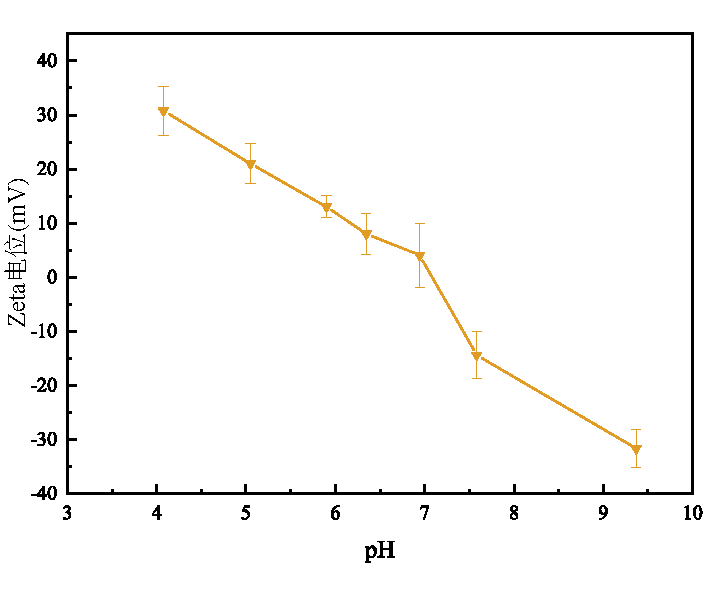
\includegraphics[width=8cm]{figs/fig3.pdf}
    \bicaption{不同pH裸S-NZVI的$\zeta$电位}{Zeta potential of bare S-NZVI as a function of pH}\label{fig3}
\end{figure}

\subsection{不同包覆比下S-NZVI的稳定性}

纳米颗粒在水中同时受到扩散和重力沉降作用,如果纳米粒子的扩散克服了沉降作用,那么纳米粒子可以保持很长时间的稳定。其中重力作用与粒子半径的平方成正比,扩散作用与粒子尺寸成反比,当纳米粒子聚集成微米大小的团簇时,由于扩散作用小于沉降作用,团聚体会沉降到容器的底部。所以沉降速率是表征S-NZVI胶体稳定性的良好指标。

\begin{figure}[h]
    \centering
    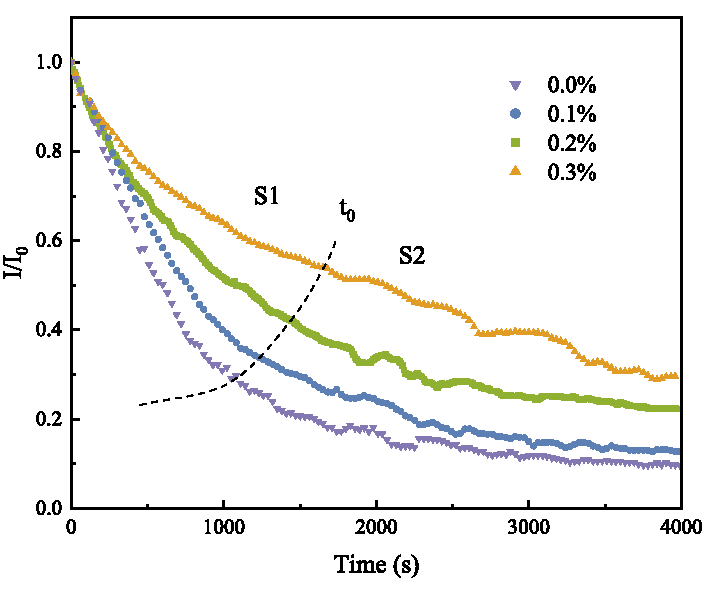
\includegraphics[width=8cm]{figs/fig1.pdf}
    \bicaption{不同包覆比和裸S-NZVI的沉降曲线}{Sedimentation curves of bare and modified S-NZVI}\label{fig01}
\end{figure}

如\cref{fig01}所示,未包覆的S-NZVI的沉降可分为两个阶段:在S1阶段,样品中存在大量超过临界尺寸的颗粒,因此快速沉降。在$t_0$时刻,多数大颗粒沉降完成,沉降速率降低,样品进入S2缓慢沉降阶段,逐渐趋于稳定。

海藻酸钠包覆S-NZVI的沉降模式与未包覆材料相同,均由S1、S2两个阶段组成,但由于聚电解质层的存在,包覆硫化钠米铁的沉降速率与海藻酸钠浓度负相关。海藻酸钠浓度越大,S1阶段的沉降速率越小,S2阶段保持悬浮的颗粒数量越多,体系的稳定性越好。

\subsection{离子强度对SA-S-NZVI稳定性的影响}

金属氧化物纳米颗粒在水溶液中的稳定性在很大程度上取决于离子强度。为了研究离子强度对SA-S-NZVI在溶液中的稳定性(pH=$8\pm 0.1$),制备不同包覆比(0、0.1、0.2、0.3wt\%)的SA-S-NZVI,采用NaCl调节离子强度(0.00$\sim$100 mM NaCl)。颗粒之间的附着效率由\cref{alpha_ppexp}计算,其中$k_{\mathrm{fast}}$取扩散限制团聚阶段下$k$的平均值。

\begin{figure}[h]
    \centering
    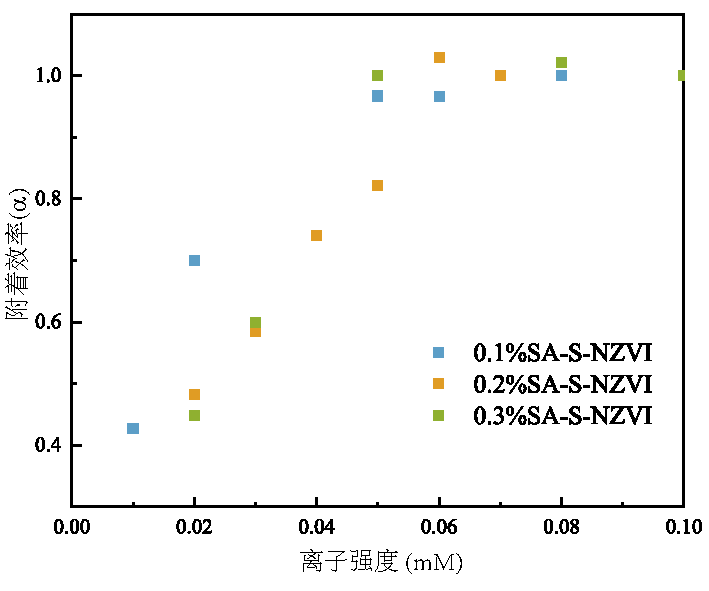
\includegraphics[width=8cm]{figs/Graph1.pdf}
    \bicaption{不同离子强度下包覆型S-NZVI的附着效率}{Influence of iron strength on aggreation behaviors of modified S-NZVI}\label{fig4}
\end{figure}

实验结果如\cref{fig4}所示,不同包覆比的SA-S-NZVI与裸S-NZVI随着离子强度的增加,在低浓度NaCl下,NaCl浓度的增加将提高电荷屏蔽的程度,从而提高团聚速率,这反映在附着效率的提高上。该过程中,附着效率与NaCl的投加量正相关,这种团聚过程称为反应限制团聚$(\alpha<1)$。在高NaCl浓度下,SA-NZVI的电荷被完全屏蔽,势垒消失,该过程中颗粒发生扩散限制团聚$(\alpha=1)$,团聚速率达到最大值,且与NaCl投加量无关。NaCl对不同包覆比S-NZVI的临界浓度均在0.05\textasciitilde0.06 mM附近。

\subsection{聚电解质包覆层的特性}

颗粒间空间斥力的大小和作用范围与表面吸附的聚合物浓度和包覆层厚度有关。不同包覆比的S-NZVI的电泳迁移率随离子强度的变化如\cref{fig5}所示,其中曲线由测量的平均电泳迁移率\cref{psidon,psi0,ue}拟合得到,各参数见\cref{tb1}。

由于包覆层的存在,SA-S-NZVI周围的扩散层被压缩,其电泳迁移率随离子强度的变化较未包覆S-NZVI小。随着离子强度不断提高,未包覆S-NZVI的电泳迁移率逐渐趋于零,而不同包覆比的SA-S-NZVI(0.1\%wt,0.2\%wt,0.3\%wt)受包覆层特性影响分别趋于-2.8,-2.2和-2.3 $\mathrm{\mu m\, s^{-1}\, cm\,V^{-1}} $。

由于软粒子对滑移面位置不敏感\cite{1992Electrophoretic},Smoluchoski公式以硬粒子为基础并不适用于包覆型S-NZVI。根据Ohshima的软粒子理论计算的包覆型S-NZVI的表面电荷$\psi_0$远小于由Smoluchoski公式计算的$\zeta$电位。因此,软粒子并不适用于传统DLVO理论的双电层公式计算静电斥力。

\begin{figure}[h]
    \centering
    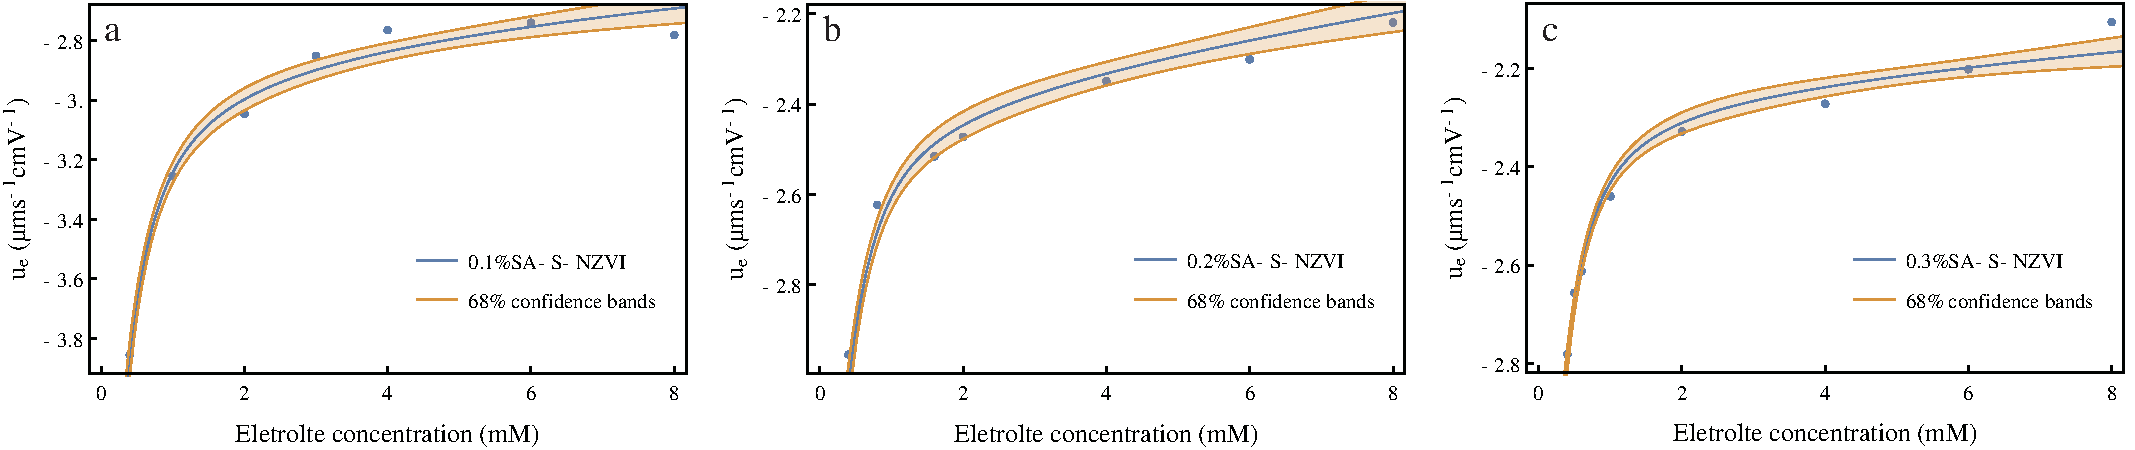
\includegraphics[width=8cm]{figs/fig5.pdf}
    \bicaption{不同NaCl浓度下包覆型S-NZVI的电泳迁移率}{Electiophoretic mobility of the sodium alginate coated S-NZVI as a function of NaCl (mM)}
    \label{fig5}
\end{figure}

\begin{table}
    \centering
    \bicaption{利用Ohshima软粒子理论计算pH值为8.0$\pm $0.1时吸附聚电解质层的特性  }{Characteristics of the adsorbed polyelectrolyte layers at pH 8.0$\pm $0.1 as estimated by Ohshima's soft particle analysis}\label{tb1}
    \begin{tabular}{@{}ccccc@{}}
        \toprule
         样品类型 & $ZN$/$\mathrm{N_A}$& $d$ & $1/\lambda$ &$\phi_p$\\
           &$(\mathrm{mol/m^3})$&(nm)&(nm)& $(10^{-3})$ \\
        \midrule
        0.1\%SA & 3.28$\pm$1.08 & 7.97$\pm$4.11 & 6.63$\pm$0.58 & 113\\
        0.2\%SA & 1.47$\pm$1.25 & 10.94$\pm$4.68 & 8.51$\pm$1.06 & 80\\
        0.3\%SA & 1.50$\pm$1.39 & 16.62$\pm$4.58 & 9.57$\pm$1.97 & 54\\
        \bottomrule
    \end{tabular}
\end{table}


包覆层中聚电解质的体积分数是影响颗粒稳定性的重要因素。根据计算的颗粒平均包覆层厚度和吸附浓度估算吸附到NZVI表面聚电解质的体积分数:

\begin{align}
    \phi_p=& \frac{\Gamma\cdot 4\pi a^2}{\rho_p\cdot \frac{4}{3}\pi [(d+a)^3-a^3]}  \\
    =&\frac{3\cdot\Gamma a^2}{\rho_p[(d+a)^3-a^3]} \nonumber
\end{align}

其中,$\rho_p$是聚电解质密度;$d$为包覆层厚度;$a$为颗粒粒径;$\Gamma$为S-NZVI表面聚电解质的吸附浓度,制备样品吸附后通过差量法利用总有机碳分析仪测量TOC计算。


\subsection{基于DLVO理论的颗粒相互作用能计算}

未包覆型S-NZVI颗粒在溶液中的稳定性可以用DLVO理论解释\cite{gregory1981approximate,bian2011aggregation}。根据经典DLVO理论,颗粒之间主要吸引能来自范德华力$V_\mathrm{vdW}$,排斥能主要取决于静电双电层的相互作用$V_\mathrm{el}$。求形颗粒之间范德华力的势能大小为\cite{huynh2011aggregation}:

\begin{equation}
    V_{\mathrm {vdW}}=-\frac{A}{6}\{\frac{2a^2}{s(4a+s)}+\frac{2a^2}{(2a+s)^2}+\ln[\frac{s(4a+s)}{(2a+s)^2}]\}
\end{equation}
其中,$A$为Hamaker常数,取$10^{-19}$;$s$为颗粒表面间距;$a$为颗粒半径。在电解质溶液中,当两个带电颗粒相互接近的时候,它们的扩散双电层彼此交迭,并且如果颗粒带电情况相似,它们在接近过程中都将受到排斥作用。根据颗粒大小和双电层厚度的不同,双电层作用$V_{\mathrm{el}}$的计算式如下\cite{bian2011aggregation,noh2010fluorescence,OHSHIMA199545}:
\begin{equation}
    V_{\mathrm{el}}=\left\{
        \begin{array}{lcl}
            4\pi \varepsilon \psi^2\cdot\frac{a_1a_2}{a_1+a_2}\cdot\ln[1+{\mathrm {exp}}(-\kappa s)]& &{\kappa a \geqslant  5}\\
            4\pi \varepsilon Y_1Y_2a_1a_2\cdot(\frac{kT}{e})^2\cdot\frac{{\mathrm {exp}}(-\kappa s)}{a_1+a_2+s}& &{\kappa a < 5}
        \end{array}\right.
\end{equation}

\begin{equation}
    \mathrm{Y_1}=\frac{8\, \tanh[e\psi /(4kT)]}{1+[1-\frac{2\kappa a_i+1}{(\kappa a_i +1)^2} \, \tanh^2[e\psi/(4kT)]] ^{1/2}} 
\end{equation}
\begin{equation}
    \kappa =\sqrt{\frac{1000 e^2 N_A I z_i^2}{\varepsilon k T}}
\end{equation}
其中,$\varepsilon$为水的介电常数,$\psi$为表面电势,未包覆型S-NZVI用$\zeta$电位$(\mathrm V)$替代\cite{wu2013aggregation,bhardwaj2010self,feriancikova2012deposition},SA-S-NZVI的表面电势由软粒子理论计算得到(\cref{tb1})。$k$为是玻尔兹曼常数$(\mathrm {J/K})$,$T$是绝对温度$\mathrm {(K)}$,$\kappa$为徳拜长度的倒数$(\mathrm m^{-1})$,$I$为离子强度$(\mathrm M)$,$e$为单电子的电荷量$\mathrm {(C)}$,$N_\mathrm{A}$为阿伏伽德罗常数$(\mathrm {mol^{-1}})$,由于体系中只有NZVI颗粒,因此$a_1=a_2$,$\mathrm{Y_1=Y_2}$。

由于S-NZVI为纳米零价铁核,表面硫化铁的核壳结构,测量S-NZVI的磁滞回线如\cref{fig6}所示,其饱和磁化强度为1410.62 kA/m,矫顽力大小为20.49 A/m,剩余磁化强度为120.08 kA/mM。因此S-NZVI在水相中的稳定性受到其固有磁矩之间相互作用的影响,即使没有外部磁场干扰,也会因NZVI自身磁矩而相互吸引\cite{butter2003direct}。考虑S-NZVI的磁性对其团聚行为的影响:

\begin{equation}
    V_\mathrm{M}=\frac{-8\pi \mu _0M^2a^3}{9(s/a+2)^3}
    \label{VM}
\end{equation}

其中,$\mu_0$为真空中磁导率$(4\pi\cdot10^{-7}H/m )$;$M$为磁化强度$(\mathrm{A\cdot m^{-1}})$。

\begin{figure}
    \centering
    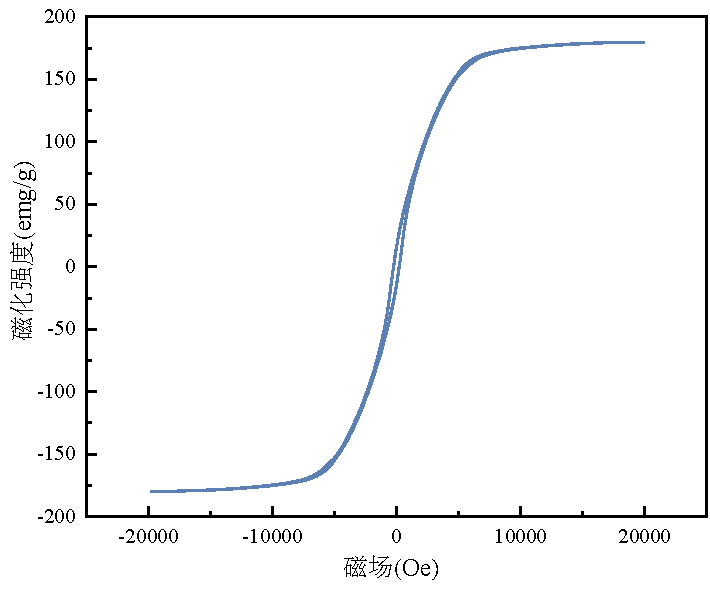
\includegraphics[width=8cm]{figs/fig6.pdf}
    \bicaption{S-NZVI在298.0 K条件下的磁滞回线}{Hysteresis cycle of the magnetization of S-NZVI, at 298.0 K.}
    \label{fig6}
\end{figure}

假设平均粒子半径为50 nm,未包覆型S-NZVI的相互作用如\cref{fig7}所示,其中$V_\mathrm{T}$为相互作用势的总和。此时相互作用力以磁力为主,不存在阻止颗粒聚集的能量势垒,颗粒快速团聚,与观察到的实验现象吻合。

\begin{figure}[h]
    \centering
    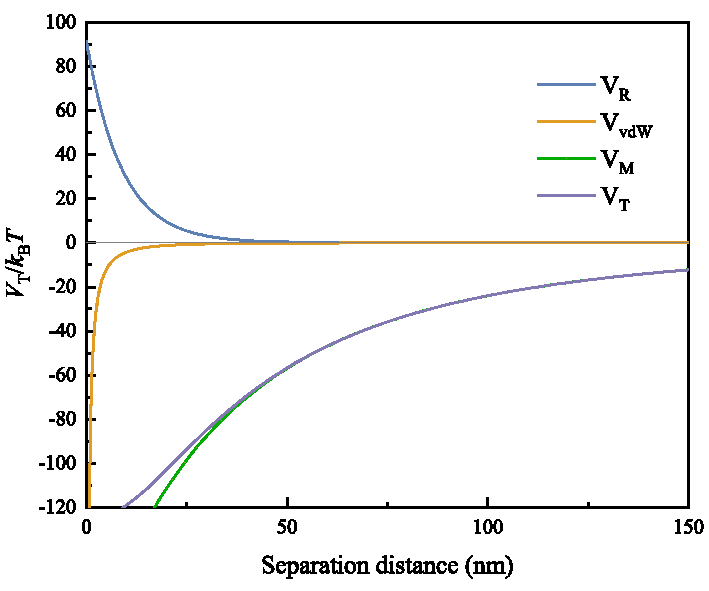
\includegraphics[width=8cm]{figs/fig7.pdf}
    \bicaption{S-NZVI的颗粒间XDLVO相互作用曲线}{Calculated XDLVO interaction energy for bare S-NZVI}
    \label{fig7}
\end{figure}

\begin{figure}[htbp]
    \centering
    \begin{subfigure}{8cm}
		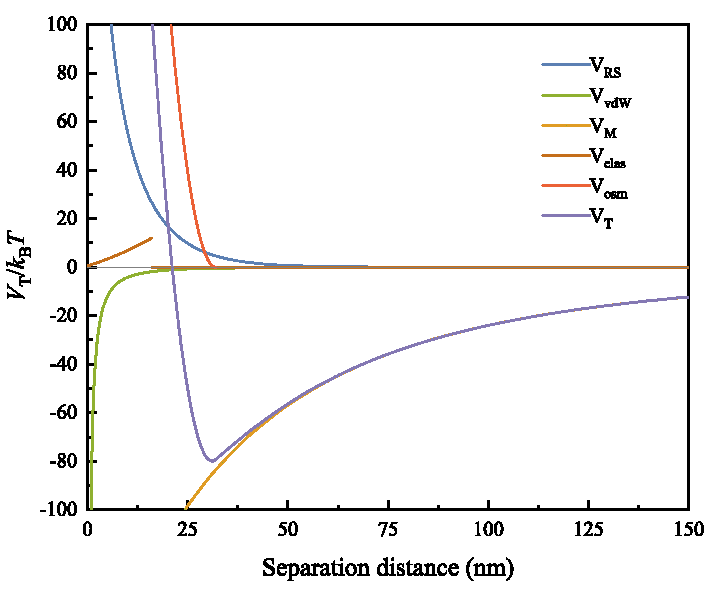
\includegraphics[width=8cm]{figs/fig8.pdf}
        \caption{0.1\%SA-S-NZVI颗粒间相互作用曲线}
        \label{fig8}
	\end{subfigure}

	\begin{subfigure}{8cm}
		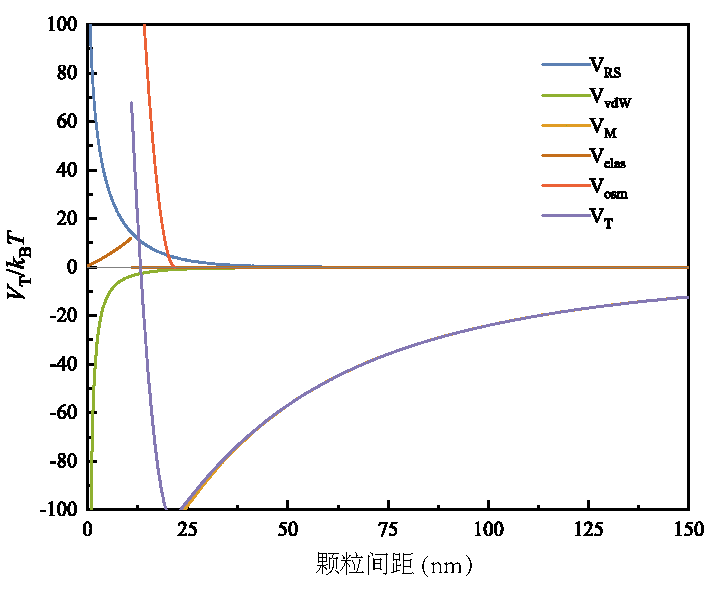
\includegraphics[width=8cm]{figs/fig9.pdf}
        \caption{0.2\%SA-S-NZVI颗粒间相互作用曲线}
        \label{fig9}
	\end{subfigure}

    \begin{subfigure}{8cm}
		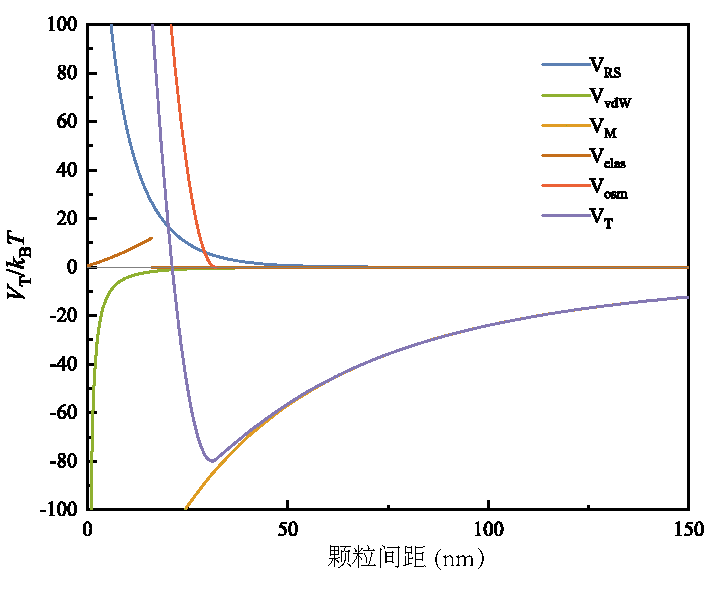
\includegraphics[width=8cm]{figs/fig10.pdf}
        \caption{0.3\%SA-S-NZVI颗粒间相互作用曲线}
        \label{fig10}
	\end{subfigure}
    \bicaption{SA-S-NZVI颗粒间相互作用曲线}{Calculated XDLVO interaction energy for SA-S-NZVI}
\end{figure}

但S-NZVI被海藻酸钠层包覆时,由于表面包覆层的存在,溶液中离子可以穿透SA-S-NZVI粒子表面分散于包覆层内部。假定包覆层是均匀带电的,令$Z$和$N$分别为包覆层中带电基团的价态和密度,则SA-S-NZVI之间的静电势为:\cite{OHSHIMA20152,vskvarla2020unified,2006390}

\begin{equation}
    V_\mathrm{els}(s)=\frac{2 \pi a \rho_\mathrm{fix}^2 \sinh^2(\kappa d)}{\varepsilon _0 \varepsilon _r\kappa ^4}\ln[\frac{1}{1-\exp(-\kappa s)}]
\end{equation}

\begin{equation}
    \rho_\mathrm{fix}=ZeN
\end{equation}

同时,根据Donnan平衡,包覆层中的聚电解质段被吸附固定在颗粒表面,而电离的小离子可以自由移动,因此包覆层附近存在额外渗透压。当颗粒间距不断减小,包覆层逐渐靠近相互重叠增加了局部电解质的浓度,从而提高了局部渗透压($V_\mathrm{osm}$)\cite{2002Electrosteric}。此外,当颗粒之间距离小于$d$时,部分聚合物段被压缩,导致体系的熵减小,从而产生弹性斥力($V_\mathrm{elas}$)\cite{doi:10.1080/07388551.2018.1440525}:

\begin{equation}
    \frac{V_\mathrm{osm}}{k_BT}=\left\{
        \begin{array}{lcl} %lcl左对齐 多行公式
            0& &{2d\leqslant s}\\
            \frac{4 \pi a }{v_1}\cdot\phi _p^2\cdot(\frac{1}{2}-\chi )(d-\frac{s}{2})^2& &{d\leqslant s <2d}\\
            \frac{4 \pi a }{v_1}\cdot\phi _p^2\cdot(\frac{1}{2}-\chi )d^2[\frac{s}{2d}-\frac{1}{4}-\ln(\frac{s}{d})]& &{s<d}
        \end{array}\right.
\end{equation}
\begin{equation}
    \frac{V_\mathrm{elas}}{k_BT}=\left\{
        \begin{array}{lcl}
            0& &{d\leqslant s}\\
            (\frac{2\pi a}{M_w}\cdot\phi_pd^2\rho_p)\{\frac{s}{d}\ln[\frac{s}{d}(\frac{3-s/d}{2})^2]\\ -6\ln(\frac{3-s/d}{2})+3(1+\frac{s}{d}^2)\}& &{d>s}
        \end{array}\right.
\end{equation}

其中,$\chi$为Flory-Huggins常数;$\phi_p$为包覆层聚电解质的体积分数;$d$为包覆层厚度;$v_1$为溶剂分子的体积;$M_w$为聚电解质的分子量;$\rho_p$为聚电解质密度。综上,包覆型S-NZVI的总相互作用能为:

\begin{equation}
   V_\mathrm{T}=V_\mathrm{vdW}+V_\mathrm{els}+V_\mathrm{osm}+V_\mathrm{elas}+V_\mathrm{M} 
\end{equation}

SA-S-NZVI的相互作用势能如\cref{fig8}所示,在短距离上看,体系中主要的排斥力为空间斥力($V_\mathrm{osm},V_\mathrm{elas}$),同时由于包覆层的存在,颗粒的表面电势($V_\mathrm{els}$)要略大于未包覆S-NZVI的静电相互作用($V_\mathrm{el}$),但是仍然无法抵抗S-NZVI自身磁矩的吸引。当SA-S-NZVI相互接近距离小于$2d$时,由于渗透斥力产生极大的能量势垒,阻止SA-S-NZVI的进一步靠近。令$V'_T=0$可求得0.3\%SA-S-NZVI的势能阱分别位于31.10 nm,大小为-79.93 $k_\mathrm{B}T$。综上,0.1 mM电解质溶液中的静电斥力无法抵抗磁力的吸引作用,颗粒主要的斥力来自于空间作用力,因此增加包覆层厚度可以显著减小势能阱的深度。对照未包覆型S-NZVI,不同包覆比的SA-S-NZVI应形成颗粒间距约31 nm的松散团聚体,而非裸S-NZVI的密实团聚体。

\begin{figure}[h]
    \centering
    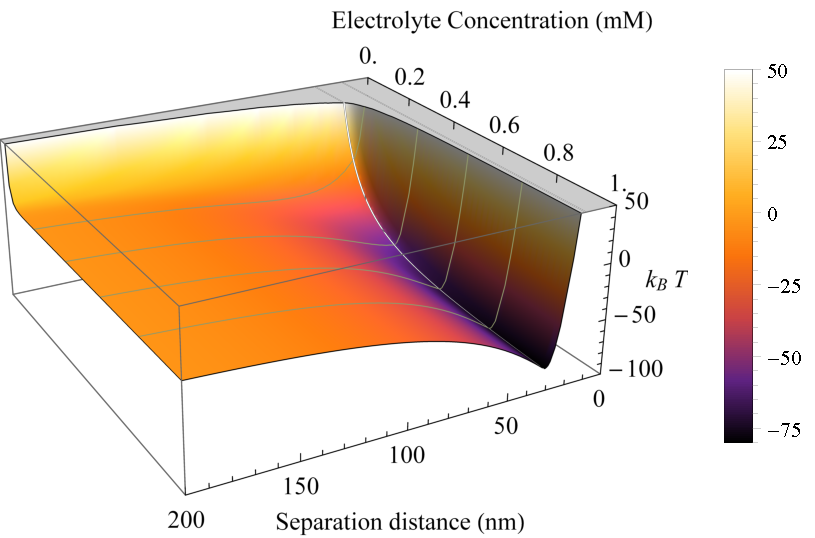
\includegraphics[width=8cm]{figs/fig11.pdf}
    \bicaption{SA-S-NZVI在不同离子强度下的总相互作用能}{Change of DLVO interaction energy for SA-S-NZVI with electrolyte concentration and separation distance}
    \label{fig11}
\end{figure}

由于SA-S-NZVI的附着效率随离子强度增加而提高(\cref{fig4}),颗粒的相互作用受离子强度影响较大。以0.3\%SA-S-NZVI为例,不同离子强度下SA-S-NZVI间的相互作用力如\cref{fig11}所示。低离子强度下颗粒间的静电斥力的大小和作用范围都显著增加,这体现在势能阱由-85.13 $k_\mathrm{B}T$(100.00 mM,图中未画出)快速衰减至-0.07 (0.01 mM)几乎消失。随着电解质浓度提高(>0.5 mM),势能阱深度的变化较小(紫色区域),静电斥力对总势能的影响变得十分有限,颗粒总势能以渗透斥力和磁力主导,最小势能阱维持在-85.13左右,离子强度对其影响可以忽略不计。同时,附着效率的物理意义为颗粒之间发生有效碰撞的几率,因此颗粒聚集的临界混凝浓度由DLVO理论计算可以表示为势能阱的深度大于布朗运动的能量(1.5 $k_\mathrm{B}T$)。要使附着效率达到100\%($\alpha_\mathrm{pp}=1$)则总势能方程需满足:

\begin{equation}
    \left\{
        \begin{array}{lcl} 
            V_T=-1.5\; k_\mathrm{B}T& \\
            V'_T=0 &
        \end{array}\right.
\end{equation}

求得不同包覆比SA-S-NZVI临界浓度分别为$4.53\cdot10^{-2}$ mM,$3.68\cdot10^{-2}$ mM,$4.47 \cdot 10^{-2}$ mM。因此三种包覆比SA-S-NZVI的附着效率在0.1 mM NaCl条件下均为100\%。利用动态光散射法测定$t_0$时刻样品的粒径分布。不同包覆比SA-S-NZVI的平均粒径随时间的变化如\cref{fig2}所示,0.1wt\%、0.2wt\%和0.3wt\%SA-S-NZVI的平均粒径分别增加了133 nm、114 nm、110 nm,可以较好的预测实验结果。

\begin{figure}[h]
    \centering
    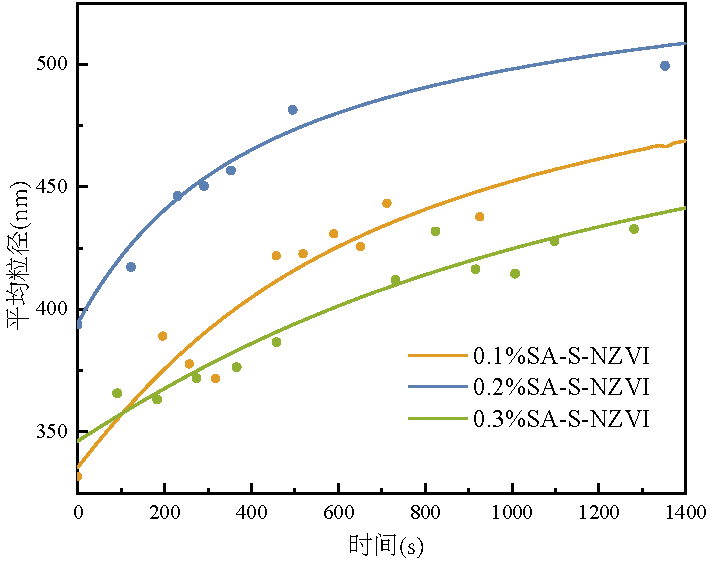
\includegraphics[width=8cm]{figs/fig2.pdf}
    \caption{Changes in mean particle size over time for suspensions of SA-S-NZVI. The curves show the best fit of the aggregation kinetics model to the 0.10 wt\%,0.2 wt\% and 0.3wt\% SA-S-NZVI}\label{fig2}
\end{figure}

为进一步研究SA-S-NZVI的团聚机理,考虑S-NZVI的长程吸引作用主要以磁力为主,而\cref{VM}计算的磁性势能与粒径的6次方正相关,而S-NZVI样品是宽分布的。因此不同粒径颗粒的总势能有显著差异。颗粒粒径,颗粒间距对总势能($V_T$)的变化如\cref{fig12}所示,由于磁性对颗粒粒径敏感,在30\textasciitilde50 nm之间,势能阱的深度随着粒径增加快速滑落,势能阱出现的位置随粒径变化较小。尺寸在30 nm以下的SA-S-NZVI颗粒的势能阱深度仅-0.82 $k_\mathrm{B}T$,小于胶体布朗运动的能量(1.5 $k_\mathrm{B}T$)。因此该条件下SA-S-NZVI形成的聚集不稳定,这可以解释沉降实验中部分SA-S-NZVI保持悬浮的现象。

\begin{figure}[h]
    \centering
    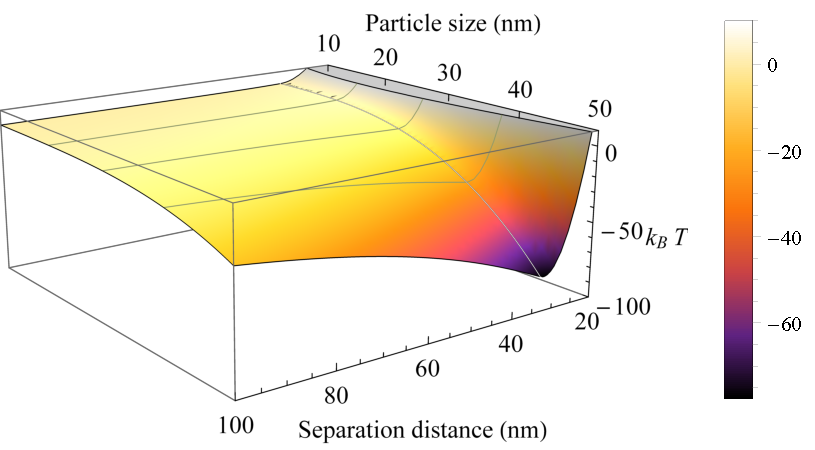
\includegraphics[width=8cm]{figs/fig12.pdf}
    \bicaption{不同离子强度下SA-S-NZVI的XDLVO相互作用}{Change of XDLVO interaction energy for SA-S-NZVI with particle size and separation distance}
    \label{fig12}
\end{figure}

\bisection{本章小结}{Result}

研究了不同的涂层比例和离子强度对裸露和涂层S-NZVI稳定性的影响。结果表明,海藻酸钠的浓度越高,沉降速度越慢。离子强度越高,粘附效率越高,离子强度对不同涂层比例的影响更可以忽略不计。通过软粒子理论计算,不同涂布比例的聚电解质层厚度分别为7.97、10.94和16.62纳米。海藻酸钠的浓度越高,聚电解质层的厚度就越大。用XDLVO理论进一步研究发现,由于S-NZVI的磁效应,颗粒总是倾向于聚结在一起。裸露的S-NZVI没有排斥性的势垒存在,所以会发生不可逆的聚集,应该会形成密集的团聚体。

相比之下,SA-S-NZVI形成31纳米的松散团聚,而不是裸S-NZVI的致密团聚。此外,虽然30纳米以下的小颗粒有结块的倾向,但吸引势能的大小远远小于布朗运动能量,这使得它难以形成稳定的结块。S-NZVI的磁效应随着颗粒间距的增加而缓慢衰减。静电排斥力和空间力的增加只能实现短距离的排斥。然而,它不能避免颗粒在长距离上相互接近的趋势。S-NZVI的磁相互作用随着粒子间距的增加而缓慢衰减。通过削弱S-NZVI的磁性或在系统中加入排斥性的长程力以匹配磁性范围,可以进一步改善S-NZVI的磁性能。

研究了不同包覆比和离子强度对未包覆和包覆型纳米颗粒稳定性的影响。结果表明,海藻酸钠浓度越高,沉降速率越慢。离子强度越大附着效率越高,同时离子强度对不同包覆比的影响较小。采用软粒子理论计算,不同包覆比分别厚度为7.97,10.94,16.62 nm。海藻酸钠浓度越高,包覆层厚度越大。用XDLVO理论进一步研究发现,由于S-NZVI的磁性作用,颗粒始终具有团聚的趋势。裸S-NZVI由于没有斥力势垒存在,发生不可逆团聚,形成密实团聚体。

相比之下,SA-S-NZVI将形成31 nm的松散团聚体,而非裸S-NZVI的致密团聚体,且颗粒尺寸在30 nm以下的小颗粒虽然具有团聚的趋势,但吸引势能远小于布朗运动能量,难以形成稳定的聚集体。而对于30 nm以上的SA-S-NZVI,虽然不可避免发生团聚,但吸引势能小,属于可逆团聚,容易被打散。因此包覆改性大大提升了S-NZVI在水中的分散能力。此外,由于S-NZVI的磁力作用随着颗粒间距增加衰减缓慢,增加静电斥力和空间作用力仅能实现短距离的排斥而无法避免颗粒长距离上相互靠近的趋势。由此可见,要实现NZVI在水溶液中真正的稳定,在后续研究中可以通过削弱S-NZVI的磁性,或在体系中增加与磁性作用范围相匹配的长程斥力以进一步提高S-NZVI的分散效果。